\section{Esercizio 1 - Analisi di algoritmi di ordinamento} 
È richiesta la realizzazione di una libreria che implementi due algoritmi di ordinamento: il Quicksort e l'Insertion sort. I due algoritmi devono essere in grado di lavorare su tipi di dati generici non specificati a tempo di compilazione della libreria.

\subsection{Implementazione}
 Per agevolare l'implementazione, la libreria definisce e si appoggia ad un tipo di dato opaco \textit{myArray}, che fornisce un set di funzioni che facilitano le operazioni su puntatori a void.\newline
Gli algoritmi di ordinamento vengono applicati ad un file csv di 20 milioni di record con 4 campi:
\begin{itemize}
    \item id: (tipo intero) identificatore univoco del record su cui non applicheremo algoritmi di ordinamento;
    \item field1: tipo intero;  
    \item field2: tipo floating point;
    \item field3: tipo stringa. Si può assumere che i valori non contengano spazi o virgole;
\end{itemize}
Il pivot del quicksort è impostato sull'elemento medio dell'array.\newline Inoltre, il quicksort è implementato nella variante 3-Way quicksort. Questa scelta è fatta per gestire l'elevato numero di valori duplicati nel dataset di prova nel campo stringa.

\subsection{Dati raccolti}
Il tempo di caricamento dei dati in memoria registrato in tabella è la media aritmetica di tutti i test fatti su quel numero di record.

\begin{table}[h]
\centering
\begin{tabular}{|c|c|c|c|c|c|c|c|}
\hline
         &           & \multicolumn{3}{c|}{\textbf{Insertion sort}} & \multicolumn{3}{c|}{\textbf{Quicksort}} \\ \hline
\textbf{elements}        & \textbf{load time} & \textbf{t(s,$f_1$)}      & \textbf{t(s,$f_2$})      & \textbf{t(s,$f_3$) }    & \textbf{t(s,$f_1$)}     & \textbf{t(s,$f_2$)}    & \textbf{t(s,$f_3$)}    \\ \hline
5000     & 0.005     & 0.060         & 0.066         & 0.121        & 0.002        & 0.001       & 0.001       \\ \hline
20000    & 0.018     & 0.987         & 0.956         & 1.711        & 0.010        & 0.016       & 0.010       \\ \hline
50000    & 0.028     & 5.852         & 7.627         & 14.180       & 0.024        & 0.029       & 0.033       \\ \hline
100000   & 0.047     & 35.211        & 40.676        & 74.151       & 0.043        & 0.068       & 0.053           \\ \hline
200000   & 0.093     & 258.125       & 282.824       & 418.370      & 0.096        & 0.116       & 0.159       \\ \hline
500000   & 0.197     & —             & —             & —            & 0.270        & 0.358       & 0.341       \\ \hline
1000000  & 0.398     & —             & —             & —            & 0.612        & 0.715       & 0.615       \\ \hline
2000000  & 0.762     & —             & —             & —            & 1.345        & 1.953       & 1.246       \\ \hline
5000000  & 1.880     & —             & —             & —            & 4.462        & 4.699       & 3.182       \\ \hline
10000000 & 4.784     & —             & —             & —            & 10.717        & 10.581       & 6.324       \\ \hline
20000000 & 9.030     & —             & —             & —            & 19.868       & 21.056      & 12.931      \\ \hline
\end{tabular}
\end{table}
\noindent
Nella tabella, $f_1$, $f_1$ ed $f_3$ si riferiscono rispettivamente al campo 1, 2 e 3 (interi, float e string).
\newline Applicando l'insertion sort su un numero superiore di 500000 record (per quanto riguarda i campi interi e float) e 200000 record (per quanto riguarda le stringhe) si ha che il tempo impiegato è superiore al tempo limite di 10 minuti. Per questo motivo si è deciso di abbandonare le misurazioni sui dati successivi.

\subsection{Analisi e considerazioni finali}
Dall'analisi dei dati raccolti in maniera sperimentale si intuisce quello che suggerisce la teoria: il quicksort è molto più veloce dell'insertion sort, come si può notare anche dal grafico qui sotto. Nonostante entrambi gli algoritmi abbiano tempo di esecuzione nel caso peggiore temporalmente uguale a $\Theta(n^2)$, il quicksort ha complessità $\Theta(n log n)$ nel caso medio. I risultati ottenuti sono concordi con quelli aspettati. \newline Inoltre, il quicksort ha tempo di esecuzione migliore sul campo stringhe, essendo l'algoritmo ottimizzato per tale caso come detto in precedenza.
\begin{figure}[h]
\centering
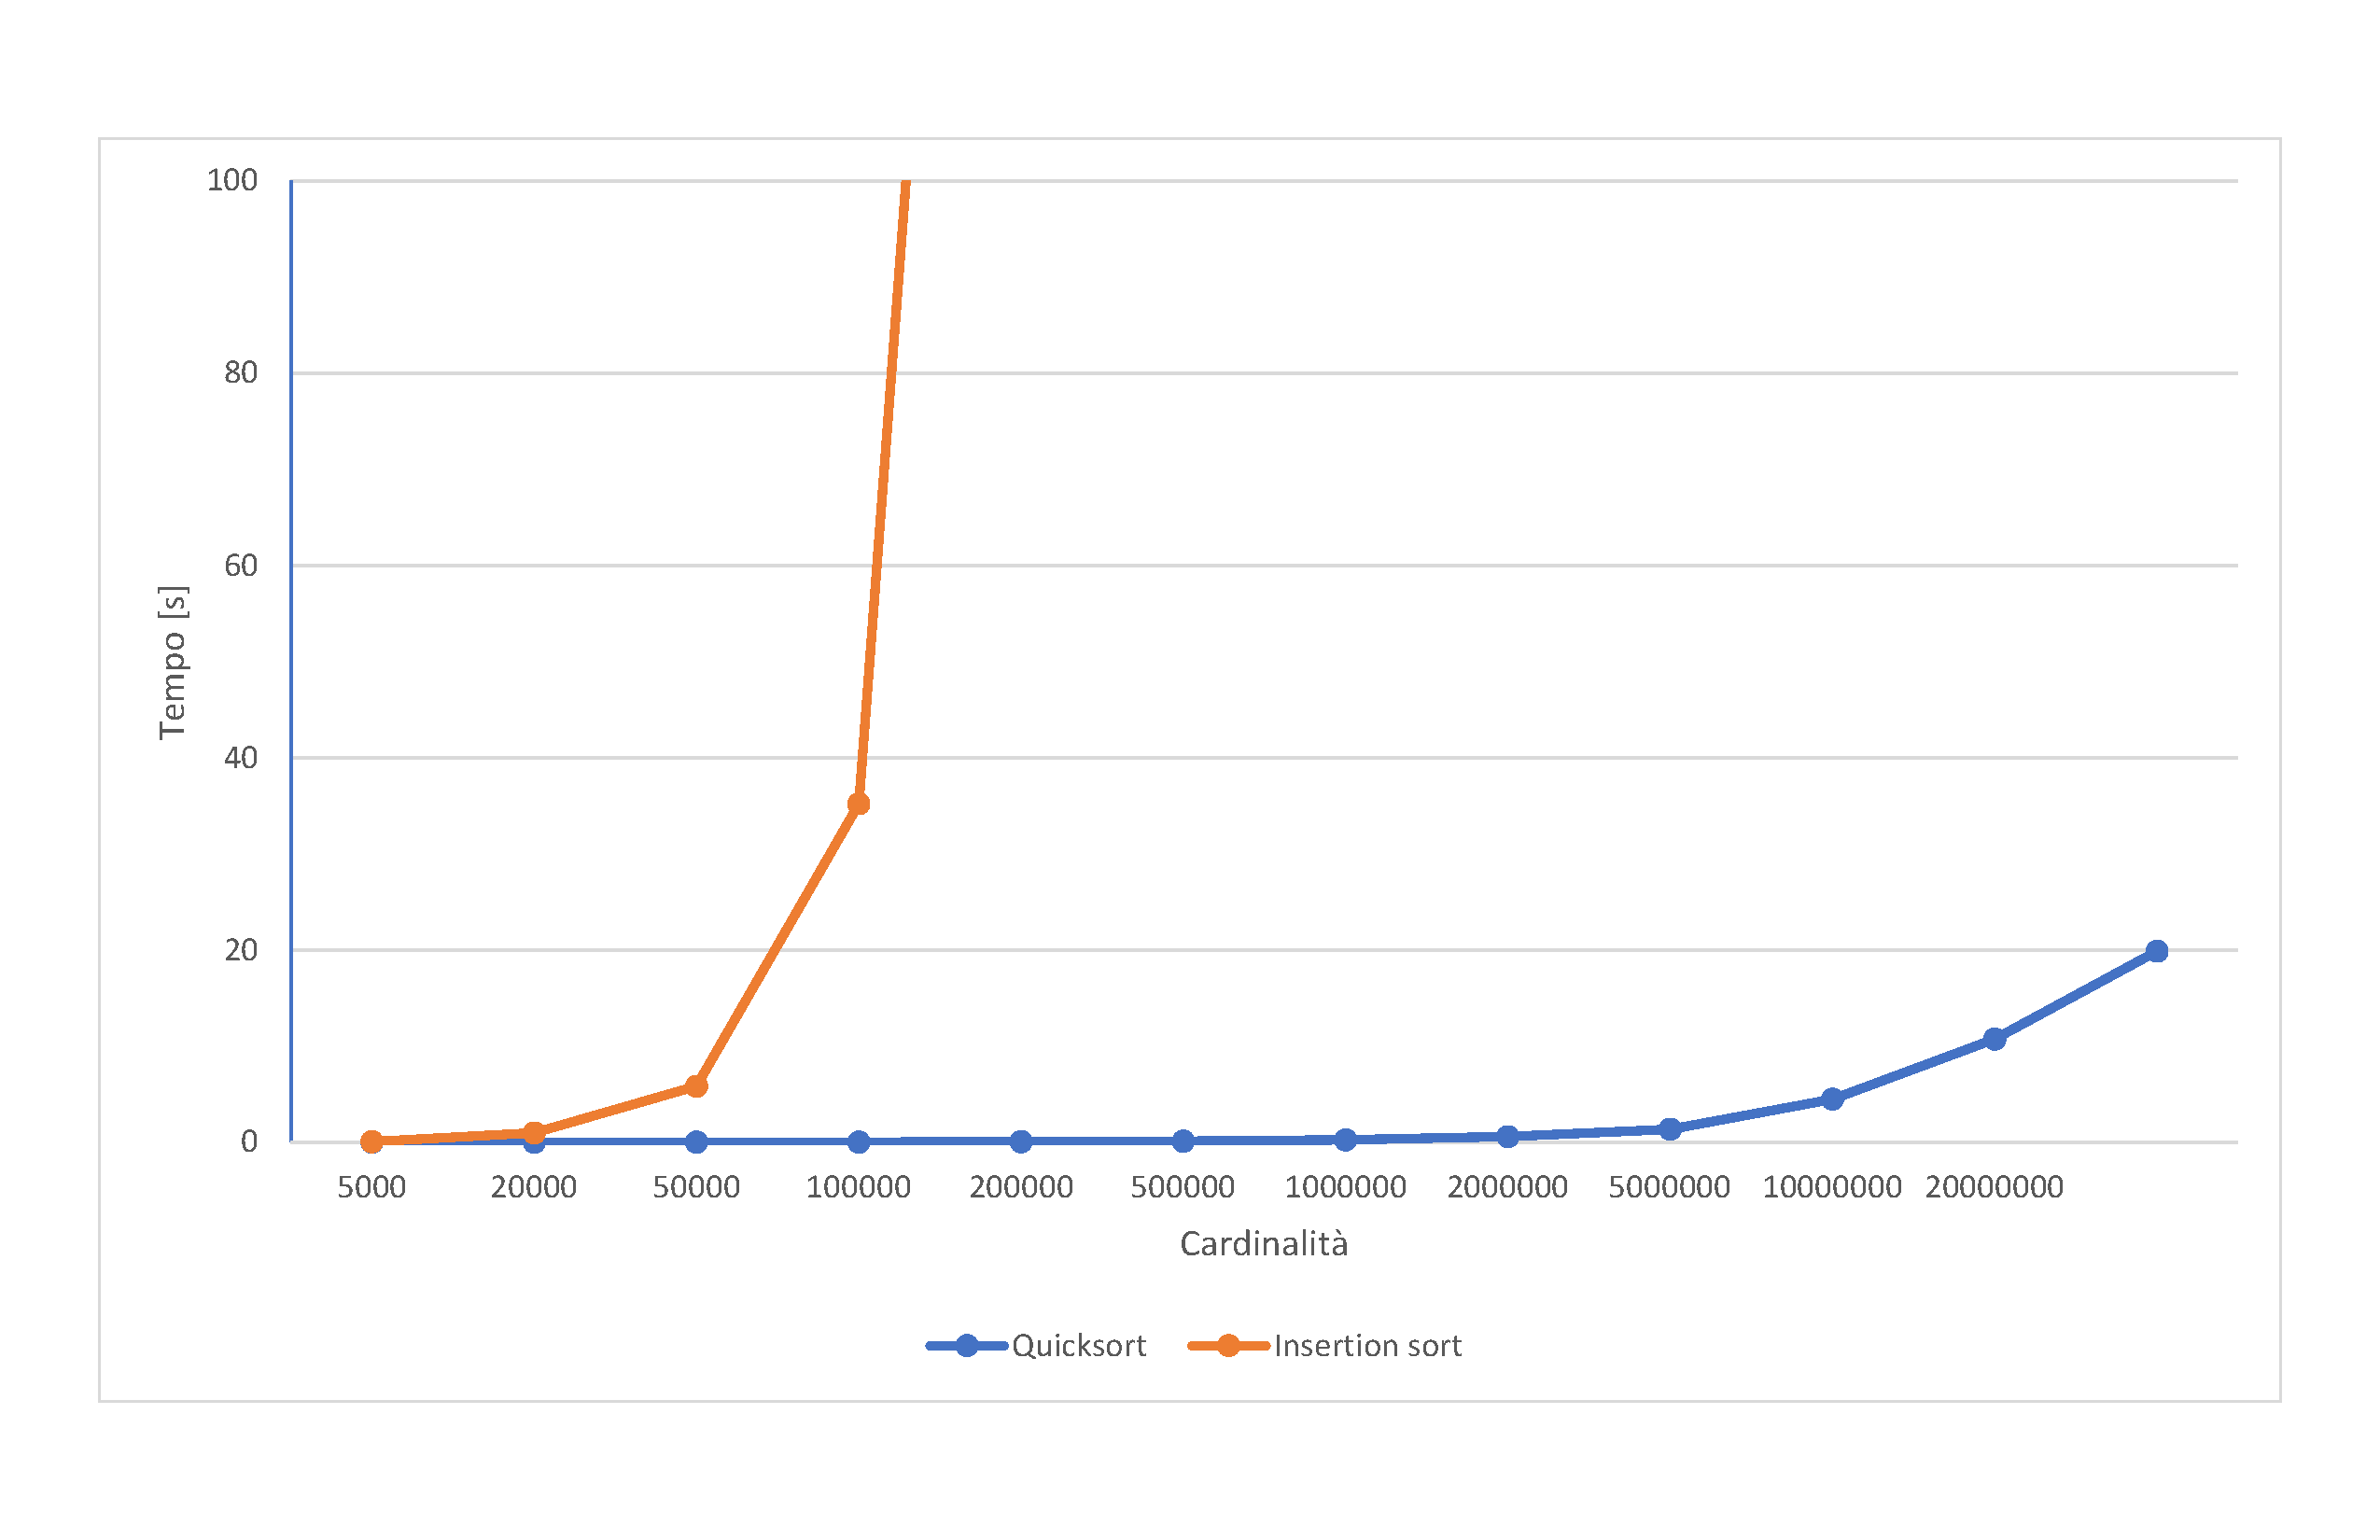
\includegraphics[trim = 21mm 30mm 56mm 37mm, clip, width=14cm]{graph.pdf}
\caption*{Andamento degli algoritmi di ordinamento in funzione al numero di elementi processati}
\label{fig:domaine}
\end{figure}